%
%  untitled
%
%  Created by Etienne van Delden on 2007-02-14.
%  Copyright (c) 2007 __MyCompanyName__. All rights reserved.
%
\documentclass{report}
\usepackage[dutch]{babel}

% Use utf-8 encoding for foreign characters
\usepackage[utf8]{inputenc}

% Setup for fullpage use
\usepackage{fullpage}
\usepackage[pdftex]{hyperref}

% Uncomment some of the following if you use the features
%
% Running Headers and footers
%\usepackage{fancyheadings}

% Multipart figures
%\usepackage{subfigure}

% More symbols
%\usepackage{amsmath}
%\usepackage{amssymb}
%\usepackage{latexsym}

% Surround parts of graphics with box
\usepackage{boxedminipage}

% Package for including code in the document
\usepackage{listings}

% If you want to generate a toc for each section (use with book)
\usepackage{minitoc}

% This is now the recommended way for checking for PDFLaTeX:
\usepackage{ifpdf}

%\newif\ifpdf
%\ifx\pdfoutput\undefined
%\pdffalse % we are not running PDFLaTeX
%\else
%\pdfoutput=1 % we are running PDFLaTeX
%\pdftrue
%\fi

\ifpdf
\usepackage[pdftex]{graphicx}
\else
\usepackage{graphicx}
\fi
\title{Gebruikershandleiding voor Hospital Manager}
\author{ OGO Groep 1b }

%\date{2007-02-14}

\begin{document}

\maketitle

\tableofcontents

\chapter{Inleiding}\label{cha:inleiding} % (fold)

Het Zorgvliet Ziekenhuis wil een informatiesysteem dat al haar
informatie koppelt en inzichtelijk maakt. Het huidige systeem
voldoet niet en er is besloten een nieuw systeem te laten maken, om
de downtime tot
een minimum te beperken.\\
Dit informatiesysteem moest voor onze ogo-opdracht, door ons worden
ontwikkeld.\\
De opdracht die door de directie van het weliswaar fictieve
Zorgvliet Ziekenhuis van grote waarde wordt geacht staat uitgebreid
gespecificeerd in de casus.\\
Dit verslag poogt een overzicht te bieden van de werkwijzen en
productontwikkelingen bij de totstandkoming van dit
informatiesysteem.\\
\\
\begin{itemize}
    \item Ontwerp\\
    In het onderdeel ``Ontwerp'' worden de Use Cases, de fictieve
    handelingen die dagelijks in het ziekenhuis voor zouden kunnen
    komen, beschreven en de bijbehorende formulieren. Tevens worden
    besluiten en aannames besproken.
    \item Modellen\\
    In het onderdeel ``Modellen'' wordt de totstandkoming van het
    ER-model besproken.
    \item Structuurbeschrijving\\
    In het onderdeel ``Structuurbeschrijving'' staan de handleiding
    van de database en drie mogelijke verbeteringen aan de database.
    \item Reflectie\\
    In het onderdel ``Reflectie'' evalueren wij elkaar en de
    opdrachten.
\end{itemize}


% chapter inleiding (end)

\chapter{Installatie}\label{cha:installatie} % (fold)

Om Hospital Manager te installeren sleept U deze uit de folder in de folder waarin U het programma wilt hebben. \\
\\
Ons programma draait alleen op Windows 2000 en hoger. MacOS X, linux en unix distributies worden niet ondersteund. Ook heeft U Microsoft Access versie 2000 of hoger nodig. Microsoft Access wordt niet met dit product meegeleverd. \\
\\
De foto's in deze handleiding kunnen afwijken van de huidige versie van Hospital Manager.


% chapter installatie (end)

\chapter{Pati\"ent}\label{cha:patient} % (fold)

U opent het pati\"entforulier door in het hoofdmenu op de knop ``Pati\"enten''
te klikken.\\
\\
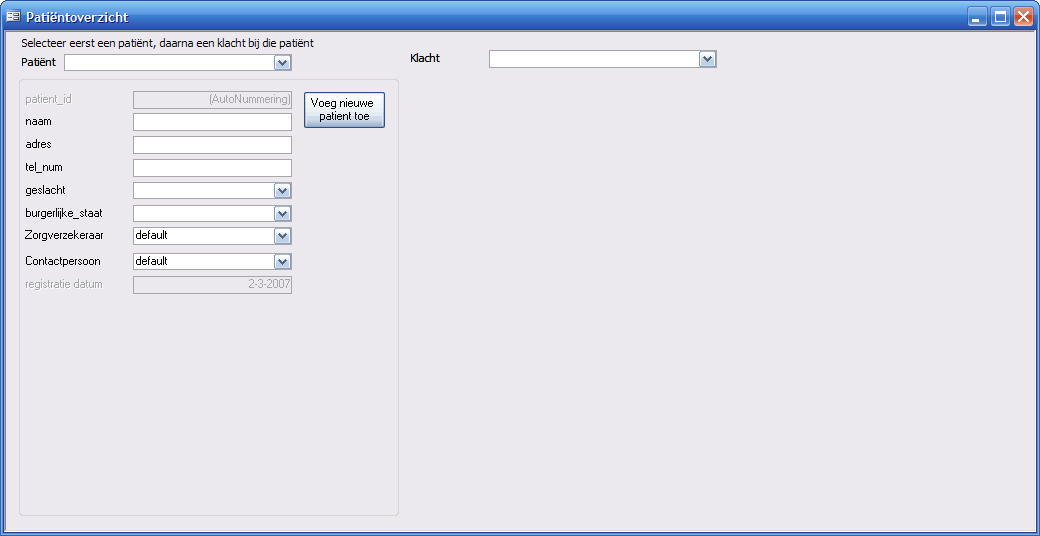
\includegraphics[scale=.5,angle=0]{patient1} \\
\\
In het pati\"entvenster venster kunt U informatie voor en over pati\"enten veranderen,
waaronder geplande opnames, pati\"entinformatie en afspraken. Ook kunt U hier recepten uitschrijven, die bij het apotheekmagazijn kunnen worden opgehaald.

\section{Pati\"entgegevens}
Als er al een pati\"ent bestaat kunt U deze selecteren uit de lijst met pati\"entnamen. Als U een nieuwe pati\"ent wilt toevoegen, klik dan op de knop ``Voeg een nieuwe pati\"ent toe'' en vul vervolgens de informatie over de nieuwe pati\"ent in.

\section{Klachten} \label{sec:klachten}
Om een pati\"ent te kunnen helpen moet de klacht geselecteerd worden uit het rechter uitrol menu. U kunt ook een nieuwe klacht aanmaken door op ``Maak nieuwe klacht aan'' te klikken. Gegevens over de klacht worden in het zonet verschenen venster ingevuld.\\
\\
Nu U de pati\"ent en een klacht heeft geselecteerd kunt U een aantal dingen
doen:
\begin{itemize}
  \item Opnames bekijken, wijzigen en inroosteren.
  \item Recepten uitschrijven, wijzigen en intrekken.
  \item Afspraken bekijken, wijzigen en aanmaken.
  \item De pati\"ent op de wachtlijst zetten voor een operatie.
\end{itemize}

\subsection{Opnames} \label{sec:opnames}
	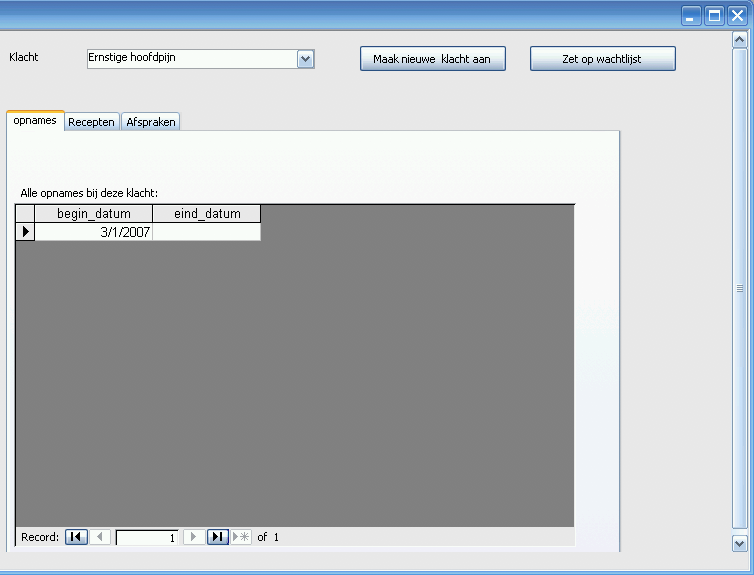
\includegraphics[scale=.5,angle=0]{patient2}\\
  \\
	Het bekijken van opnames doet U door op het tabblad ``Opnames''
        te klikken. Hier staan alle (geplande) begin- en eindtijden van de
	opnames van een pati\"ent. Door op het plusje te klikken voor een
	afspraak, kunt U bekijken (en toevoegen) op welke bedden een pati\"ent
	heeft gelegen tijdens een opname. Elk bed staat op een andere afdeling.

% subsection opnames (end)

\subsection{Recepten} \label{sec:recepten}
	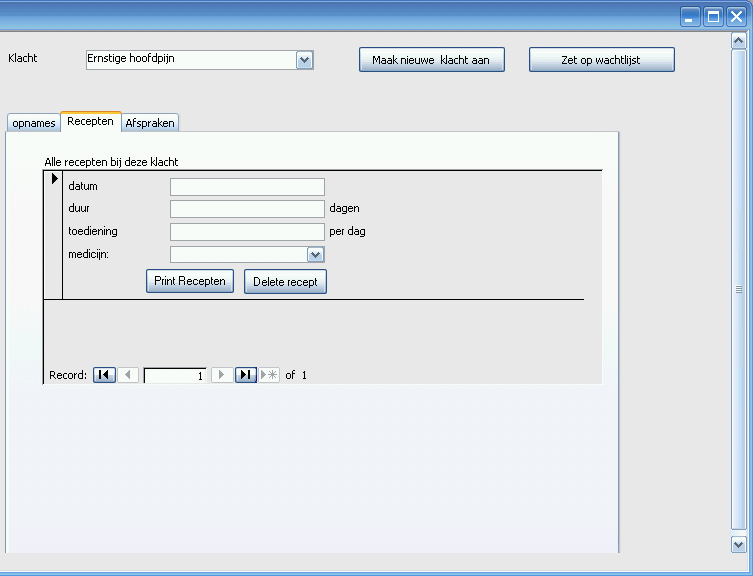
\includegraphics[scale=.5,angle=0]{patient3}\\
  \\
	Het bekijken van recepten doet U door op het tabblad recepten
        te klikken. Hier kunt U recepten bekijken en uitschrijven met de knoppen
	``Print Recepten'' en ``Delete Recept''. Met de pijltjes
	kunt U bladeren door de verschillende recepten bij de geselecteerde klacht.
	
% subsection recepten (end)

\subsection{Afspraken} \label{sec:afspraken}
  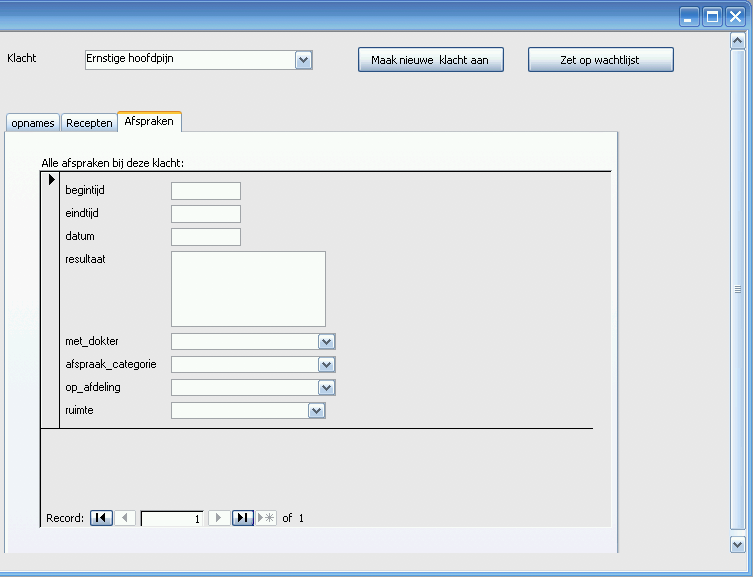
\includegraphics[scale=.5,angle=0]{patient4}\\
  \\
  Het bekijken van afspraken doet U door op het tabblad
	``Afspraken'' te klikken. Hier kunt U de afspraken voor de huidige pati\"ent bekijken	(via de pijltjes onderaan). Ook kunt U een nieuwe afspraak	aanmaken door op het ``nieuwe record'' knopje (met het pijltje sterretje symbool) te klikken.

% subsection afspraken (end)

\subsection{Wachtlijst} \label{sec:wachtlijst}
	U kunt een pati\"ent voor operatie op de wachtlijst zetten met de knop ``Zet
	op wachtlijst'' waarna automatisch de juiste pati\"ent en case wordt geselecteerd,
	zie hiervoor verder de handleiding voor het venster wachtlijst.

% subsection wachtlijst (end)

% section klachten (end) 

% chapter patient (end)


\chapter{Opnames}\label{cha:opnames} % (fold)

Onder de knop ``Opnames'' vindt U een overzicht van de pati\"enten
die in het ziekenhuis aanwezig zijn, in het verleden zijn opgenomen
of die ingepland zijn om in de toekomst opgenomen te worden.\\
\\
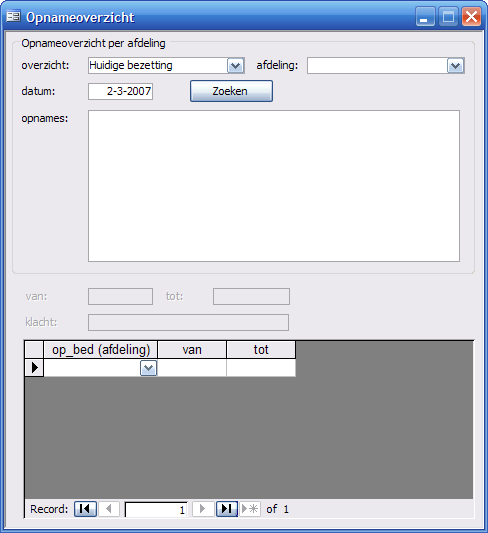
\includegraphics[scale=.5]{opnames1}

\section{Opnameoverzicht}\label{sec:opnameoverzicht} % (fold)

Er kunnen verschillende typen overzichten worden weergegeven. Kies
een type overzicht uit de lijst. Hieronder wordt meer uitgelegd over
de verschillende typen overzichten.

% section opnameoverzicht (end)

\section{Overzicht selecteren}\label{sec:overzicht selecteren} % (fold)

Om een overzicht van opnames te maken wordt er een datum ingevuld en
optioneel een afdeling. Als de naam van een afdeling wordt ingetypt
of geselecteerd uit een lijst, dan worden alleen de opnames van die
afdeling weergegeven. Als het tekstvak voor de afdeling wordt
leeggelaten, dan worden de opnames voor alle afdelingen weergegeven.
Om de pati\"enten weer te geven klikt U op de knop ``Zoeken''.

% section overzicht selecteren (end)

\section{Overzichtstypen}\label{sec:overzichtstypen} % (fold)

Er zijn vijf typen overzicht:
\begin{itemize}
  \item Huidige bezetting
  \item Huidige opnames
  \item Huidige ontslagen
  \item Afgehandelde opnames
  \item Toekomstige opnames
\end{itemize}

\subsection{Huidige bezetting}\label{sec:huidige bezetting} % (fold)
Alle pati\"enten die op de opgegeven datum in het ziekenhuis of op de geselecteerde afdeling aanwezig zijn worden weergegeven.
\subsection{Huidige opnames}\label{sec:huidige opnames} % (fold)
Alle pati\"enten die op de opgegeven datum in het ziekenhuis of op de geselecteerde afdeling opgenomen zullen worden.
\subsection{Huidige ontslagen}\label{sec:huidige ontslagen} % (fold)
Alle pati\"enten die op de opgegeven datum uit het ziekenhuis of van de geselecteerde afdeling ontslagen zullen worden.
\subsection{Afgehandelde opnames}\label{sec:afgehandelde opnames} % (fold)
Alle pati\"enten die voor de opgegeven datum in het ziekenhuis of op de geselecteerde afdeling een opname hebben gehad en zijn ontslagen.
\subsection{Huidige bezetting}\label{sec:huidige bezetting} % (fold)
Alle pati\"enten die op de opgegeven datum nog niet in het ziekenhuis of op de geselecteerde afdeling opgenomen zijn en waarvoor in de toekomst een opname gepland staat.

% section overzichtstypen (end)

\section{Detailvenster}\label{sec:detailvenster} % (fold)

Details over de opnames bij de case waarvoor de geselecteerde
pati\"ent is opgenomen kunnen in het detailvenster worden bekeken en
aangepast.

% section detailvenster (end)


% chapter opnames (end)


\chapter{Wachtlijst}\label{cha:wachtlijst} % (fold)

U opent het wachtlijst venster door in het hoofdmenu op de knop ``Wachtlijst'' te klikken. Het wachtlijst venster bestaat uit een aantal knoppen,
	waarmee U de wachtlijst kunt bekijken en manipuleren.
	Op de wachtlijst zelf staan mensen die geopereerd moeten worden,
	maar die nog niet ingepland zijn.\\
\\
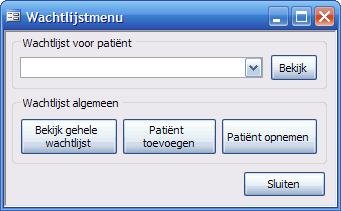
\includegraphics[scale=.7]{wachtlijst1}

\section{Wachtlijst bekijken} \label{sec:wachtlijst bekijken}
	Met de knop ``Bekijk gehele wachtlijst'' krijgt U een lijst met alle mensen op de wachtlijst. Om per pati\"ent deze wachtlijst te bekijken selecteert U in het gebied ``Wachtlijst voor pati\"ent'' een pati\"ent uit het uitrol menu en klikt U vervolgens op de knop ``Bekijken''. Met de twee andere knoppen kunt U pati\"enten aan de wachtlijst toevoegen of op laten nemen.\\

\section{Aan wachtlijst toevoegen} \label{sec:toevoegen}
	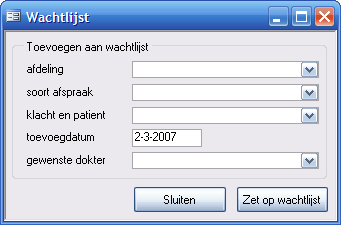
\includegraphics[scale=.6]{wachtlijst2}\\
  \\
	De knop ``Zet op wachtlijst'' opent een venster waarin U een pati\"ent en een klacht selecteert, het gewenste type operatie en de dokter die gaat opereren. Als alles naar wens is ingevuld
	klikt U op de knop ``Zet op wachtlijst''.
	
\section{Van wachtlijst tot opname} \label{sec:opname inplannen}
	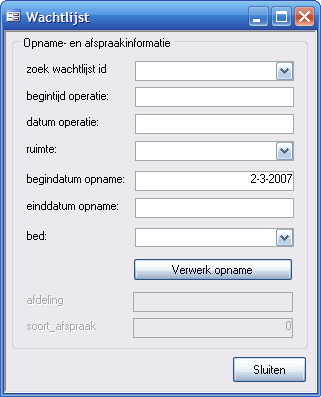
\includegraphics[scale=.6]{wachtlijst3}\\
  \\
	Als er plaats in het ziekenhuis is vrijgekomen kunnen er nieuwe pati\"enten vanaf de wachtlijst worden opgenomen. Met het wachtlijstnummer kunt U makkelijk zoeken naar personen die op de wachtlijst staan. Met de knop ``Verwerk opname'' wordt een pati\"ent van de wachtlijst gehaald en er wordt een opname ingepland \'en een afspraak voor een operatie gemaakt. Dit gaat als volgt: In een nieuw venster krijgt U een rapport te zien waarin U een beter overzicht van de complete wachtlijst krijgt. Ook kunt U informatie invullen over de operatie en de opname van de pati\"ent.



% chapter wachtlijst (end)

\chapter{Rekeningen}\label{cha:rekeningen} % (fold)

U opent het rekeningformulier door in het hoofdmenu op de knop ``Rekeningen'' te klikken. U kunt in dit formulier rekeningen opmaken per pati\"ent of per afdeling. Het formulier bestaat uit een aantal knoppen waarmee U rekeningen kuntbetalen, bekijken en versturen. Hieronder wordt uitlegd hoe dit in zijn werk gaat.\\
\\
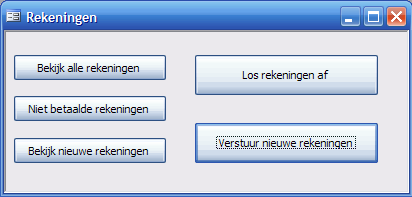
\includegraphics[scale=.8]{rekeningen1}

\section{Rekeningen bekijken} \label{sec: niewe rekeningen}
U kunt de rekeningen bekijken met de knop ``Bekijk alle rekeningen''.
De knop ``Niet betaalde rekeningen'' laat hetzelfde rapport zien, maar
dan alleen met de rekeningen die niet betaald zijn.

\section{Nieuwe rekeningen} \label{sec: nieuwe rekeningen}
Met de knop ``Bekijk nieuwe rekeningen'' kunt U nieuwe rekeningen bekijken en versturen. Door
ze te bekijken opent U een preview met alle nieuwe rekeningen. Door ze te
versturen worden ze opgeslagen in de database en verstuurd op de huidige
datum.

\section{Rekeningen aflossen} \label{sec:rekeningen aflossen}
De knop ``Los rekening af'' opent een venster waarin U een rekening (bij een pati\"ent)
kunt selecteren en vervolgens het uitstaande bedrag (wat al betaald is) kunt
bijwerken met de knop ``Betaal'', nadat U heeft ingevuld hoeveel de patient
betaald heeft.

% chapter rekeningen (end)

\chapter{Werknemer}\label{cha:werknemer} % (fold)

U komt in het werknemersscherm door in het hoofdmenu op de knop ``Werknemers''
te klikken.\\
\\
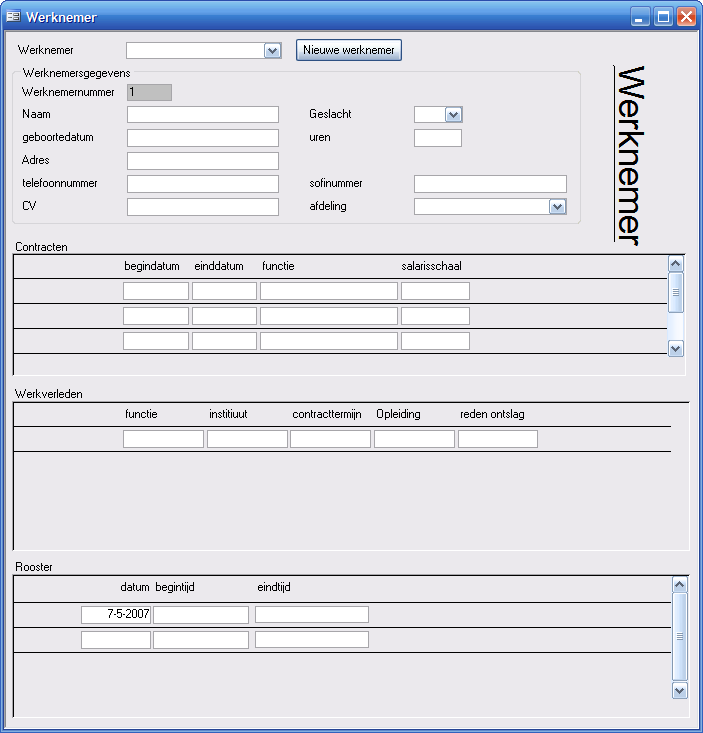
\includegraphics[scale=.5]{werknemer2} \\
\\
Selecteer bovenin het scherm een bestaande werknemer. U kunt ook een nieuwe werknemer aanmaken door op de ``Nieuwe
werknemer'' knop te klikken en vervolgens de juiste informatie in te voeren.

\section{Werknemersgegevens} \label{sec:werknemersgegevens}
    Onder het werknemersselectieveld staan de persoonsgegevens
    van de werknemer. Gebruik dit gebied om zaken als adresgegevens
    te wijzigen.

% subsection werknemersgegevens (end)

\section{Contracten} \label{sec:contracten}
    In het gebied ``contracten'' wordt op elke rij een contract
    van de werknemer bij het Zorgvliet Ziekenhuis weergegeven. Het
    huidige contract heeft geen einddatum. Om een contract toe te voegen, typt U de gegevens over dat
    contract in op de onderste regel. Er wordt dan automatisch een nieuwe lege regel aangemaakt.

% subsection contracten (end)

\section{Werkverleden} \label{sec:werkverleden}
    In het gebied ``werkverleden'' wordt op elke regel informatie over een
    opleiding of werkervaring van een werknemer buiten het Zorgvliet Ziekenhuis bijgehouden.
    Om een type werkervaring of opleiding toe te voegen, typt U de
    gegevens over die opleiding of werkervaring in op de onderste
    regel. Er wordt dan automatisch een nieuwe lege regel aangemaakt.

% subsection werkverleden (end)

\section{Rooster} \label{sec:rooster}
    In het gebied ``rooster'' wordt het rooster van een
    werknemer bijgehouden. Op elke regel staat een dienst van de
    werknemer. Om een dienst toe te voegen, typt U de gegevens in op een lege
    regel. Er wordt dan automatisch een nieuwe lege regel toegevoegd.

% subsection rooster (end)


% chapter werknemer (end)

\chapter{Afspraken}\label{cha:afspraken} % (fold)

U kunt een overzicht van afspraken opzoeken door middel van het afspraken venster, die U kunt openen door op  ``Afspraken'' te klikken.\\
\\
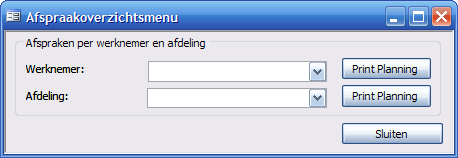
\includegraphics[scale=.7]{afspraken1}

\section{Afspraken per werknemer}\label{sec:per werknemer}

Selecteer de naam van een werknemer uit het uitrol menu en klik op de knop ``Print planning''.

\section{Afspraken per afdeling}\label{sec:per afdeling}

Selecteer de naam van een afdeling uit het uitrol menu en klik op de knop ``Print planning''.

% chapter afspraken (end)


\chapter{Magazijn}\label{cha:magazijn} % (fold)

Onder de knop ``Magazijn'' kunt U de totale verbruikte producten per
pati\"ent of per afdeling vinden. Hieronder zullen we uitleggen hoe
dit in zijn werk gaat.\\
\\
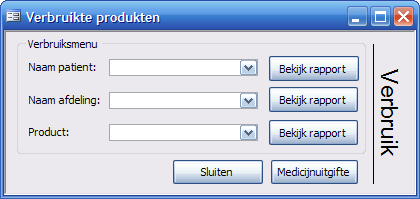
\includegraphics[scale=.7]{magazijn1}

\section{Verbruik per pati\"ent}\label{sec:verbruik_per_pati_ent} % (fold)

Voor het verbruik per pati\"ent selecteert U de patient door zijn
naam in het aangegeven veld te tikken of deze te selecteren uit de
lijst. Vervolgens klikt U op ``Bekijk rapport''. Een nieuw venster
verschijnt met de gevraagde gegevens.

% section verbruik_per_pati_ent (end)

\section{Verbruik per afdeling}\label{sec:verbruik_per_afdeling} % (fold)

Voor het verbruik per afdeling selecteert U de afdeling door die in
het aangegeven veld te tikken of deze te selecteren uit de lijst.
Vervolgens klikt U op ``Bekijk rapport''. Een nieuw venster
verschijnt met de gevraagde gegevens.

% section verbruik_per_afdeling (end)

\section{Verbruik per product}\label{sec:verbruik_per_product} % (fold)

Voor het verbruik per product selecteert U het product door die in
het aangegeven veld te tikken of deze te selecteren uit de lijst.
Vervolgens klikt U op ``Bekijk rapport''. Een nieuw venster
verschijnt met de gevraagde gegevens.

% section verbruik_per_product (end)

\section{Medicijnuitgifte}\label{sec:uitgifte van medicijnen} % (fold)

Om medicijnen uit te geven klikt U op de knop ``Uitgiftes''.
Onderstaand venster wordt geopend. Er worden namen van pati\"enten
weergegeven die \'e\'en of meerdere openstaande recepten hebben. De
openstaande recepten van een pati\"ent staan op datum gesorteerd.\\
\\
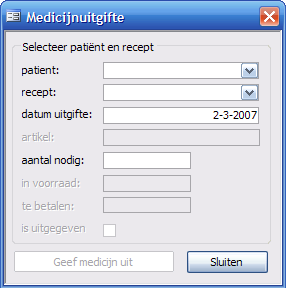
\includegraphics[scale=.7]{uitgifte1}

\subsection{Recept selecteren}\label{sec:recept selecteren} % (fold)

Selecteer de pati\"ent aan wie U een medicijn wilt uitgeven door de
naam in te typen of te selecteren uit de lijst. Selecteer vervolgens
de datum waarop het recept is voorgeschreven door de datum in te
typen of te selecteren uit de lijst. De naam van het medicijn waar
het recept voor is staat aangegeven naast de datum van uitgifte van
het recept.

\subsection{Datum van uitgifte}\label{sec:datum van uitgifte} % (fold)

De datum van uitgifte staat standaard ingesteld op de huidige datum,
maar deze kan aangepast worden, dit in verband met administratie van
eerder uitgegeven medicijnen die nog niet geregistreerd waren.

\subsection{Aantal eenheden}\label{sec:aantal eenheden} % (fold)

Het aantal eenheden medicijn dat moet worden uitgegeven wordt
automatisch berekend aan de hand van het recept. Mocht er toch een
aantal eenheden medicijn meer meegegeven moeten worden (bijvoorbeeld
omdat er per doosje meer eenheden verpakt zitten dan nodig voor de
pati\"ent) dan kan dit berekende aantal nog handmatig worden
aangepast.

\subsection{Uitschrijven}\label{sec:Uitschrijven} % (fold)

Om het medicijn uit te schrijven klikt U op de knop ``Geef medicijn uit''. Wanneer de gevraagde hoeveelheid medicijn in de
voorraad aanwezig is wordt het medicijn aan de klant meegegeven en
wordt de voorraad bijgewerkt. Het recept kan dan ook niet meer
worden uitgegeven en zal niet meer in de lijst met uitgeefbare
medicijnen te zien zijn. Als het medicijn niet voldoende op voorraad
is, kunt U het medicijn niet uitgeven en kan de pati\"ent het
medicijn op een later tijdstip komen ophalen. Het venster wordt
automatisch gesloten.

% section uitgifte (end)


% chapter magazijn (end)

\chapter{Beveiliging}\label{cha:beveiliging} % (fold)

\input{beveiliging}

\bibliography{}
\end{document}
